\documentclass{template}
\usepackage{enumitem}

\newcommand{\version}{Version 1.3}
\author{Denis Ivan Blazevic, \url{denbl369@student.liu.se}\\
  Frans Bergström, \url{frabe808@student.liu.se}\\
    }
\title{Kravspecifikation}
\date{2016-11-08}
\rhead{Denis Ivan Blazevic\\
Frans Bergström\\
}


\begin{document}
\projectpage

\tableofcontents
\newpage

\section{Revisionshistorik}
\begin{table}[!h]
\begin{tabularx}{\linewidth}{|l|X|l|}
\hline
Ver. & Revisionsbeskrivning & Datum \\\hline
1.3 & Ändrat enligt statusrapporter & 161219 \\\hline
1.2 & Reviderat enligt feedback från handledaren & 161123 \\\hline 
1.1 & Reviderat enligt feedback från beställargrupp & 161115 \\\hline 
1.0 & Första versionen av kravspecifikationen. & 161108 \\\hline
\end{tabularx}
\end{table}


\section{Spelidé}
En spelare ska styra ett spelobjekt som är avbildat som en student som går på Innovativ Programmering på Linköpings Universitet. Spelaren styr `studentens' hastighet och vilket spår som `studenten' ska gå i, samtidigt som `studenten' bär på en kopp kaffe. Spelet är inspirerad av runner spel såsom Temple Run fast från en top-down vy och med en egen twist på det. Spelaren måste balansera kaffet så att det inte spills under spelets gång. Det kommer att finnas hinder i form av `halt golv', `studenter som ligger ner på marken', och andra studenter som går mot spelaren. 

Målet med spelet är att gå från Café Java till Grottan/Playan med en kopp kaffe utan att spilla allt, detta kommer vara tajmat och skrivas in på en poängtavla (som innehåller sluttid och mängd kaffe kvar) i slutet av spelet. Kaffet måste balanseras, vilket blir jobbigare desto fortare spelaren väljer att gå. De olika hinder som dyker upp kommer att sega ner spelaren, eller få denna att spilla lite av kaffet om spelaren inte reagerar i tid. Slutpoäng räknas i form av sluttid och mängd kaffe kvar. 

\subsection{Svårighetsgrad}
Spelets svårighetsgrad kommer variera på hur spelaren väljer att spela. Vill denne slå rekordet tidsmässigt, kommer spelet vara mycket svårare då farten av `studenten' kommer att få kaffet att vara svårbalanserat. De olika hinder kommer även sega ner spelaren OM spelaren inte väljer att springa rakt över dem - detta kommer bidra till att liten del av kaffet spills men spelaren vinner på tid. Detta betyder dock inte att spelaren kan bara springa igenom banan och spilla hur mycket som helst då rekordet är inte bara tidsmässigt men även hur mycket kaffe som är kvar. Om inget kaffe är kvar, förlorar spelaren automatiskt.

\section{Målgrupp}
Spelet riktar sig till alla som är intresserade av enkla arkadliknande spel med enkla principer. Spelet är även väldigt riktat till studenter på Innovativ Programmering.

\section{Spelupplevelse}
Spelet kommer variera mellan att vara stressfullt och relativt enkelt, beroende på spelarens vilja. Ju snabbare spelaren väljer att gå framåt, desto mer poäng kommer denne att få baserat på tid och kaffespill.

\pagebreak

\section{Spelmekanik}
Spelplanen är statisk, men hinder genereras vid start av spelomgång. Spelaren navigerar spelplanen genom att trycka på de knappar som får `studenten' att ändra hastigheten eller röra sig åt sidorna. Spelaren har en kaffemätare och en uthållighetsmätare. Beroende på spelarens fart går uthållighetsmätaren ner, för att kontra det måste spelaren dricka kaffet, men på så sätt går kaffet åt och därför sänks kaffemätaren. En hastighetsmätare kommer finnas som visar spelarens maxhastighet, går spelaren över denna maxhastighet snubblar spelaren och förlorar. Spelaren kan kolla ner för att undvika ögonkontakt med andra studenter som går mot spelaren.

Spelaren kommer inte behöva hantera svängar manuellt, spelet kommer sköta det åt spelaren genom att vända på `studenten' och spelplan åt rätt håll. När spelaren kommer fram till Grottan/Playan (markeras i spelvärlden med målflaggor) kommer spelarens poäng visas upp och sedan kommer poängtavlan visas upp. Vi kommer använda en algoritm för att räkna ut spelarens totala poäng där vi använder kaffet och tiden som parametrar. Vår algoritm i nuläget ser ut som följande: slutpoäng = (tid i sekunder/kaffet i procent), där spelaren ska sträva efter att få så lågt slutpoäng som möjligt.
\\Se Tabell 1 för en överblick över de knappar som kommer användas.


\begin{table}[]
    \centering
    \caption{Tangentknappar}
    \label{mekanik}
    \begin{tabular}{|l|l|}
        \hline
        \multicolumn{1}{|c|}{\textbf{Tangentknapp}} & \multicolumn{1}{c|}{\textbf{Åtgärd}} \\ \hline
        A & Byter till spår åt vänster. \\ \hline
        D & Byter till spår åt höger. \\ \hline
        W & Ökar hastigheten. \\ \hline
        S & Sänker hastigheten. \\ \hline                
        Vänster-pil & Balansera kaffe koppen till vänster. \\ \hline
        Höger-pil & Balansera kaffe koppen till höger. \\ \hline
        Ner-pil & Kolla ner i marken. \\ \hline
        Upp-pil & Dricka kaffe. \\ \hline        
        Space & Hoppa. \\ \hline
        ESC & Pausa spelet / visa menyn. \\ \hline
    \end{tabular}
\end{table}

\section{Regler}
\subsection{Allmänt}
\begin{itemize}
\item Spelaren har begränsat kaffe i kaffekoppen. Kaffe kan inte fyllas upp igen.

\item Om spelaren kolliderar med ett hinder, spills en del av kaffe beroende på `studentens' fart, och beroende på hindret så ska `studenten' trilla och förlora all sin fart - men spelaren förlorar inte spelet.

\item Om spelaren går för fort på halt golv, spills en större del av kaffet och `studenten' förlorar spelomgången.

\item Om spelaren inte kollar bort från en annan student som går mot spelaren, kommer spelaren inte kunna röra sig på fem sekunder. När spelaren kollar bort från en annan student, blir skärmen svart i två sekunder.
\item Om spelaren har slut på kaffe eller springer för fort, förlorar spelaren.

\end{itemize}
\subsection{Spelplanen}
\begin{itemize}
\item `Studenten' kommer att röra sig framåt (riktning upp på dataskärmen.).
\item Spelplanen ska innehålla tre olika spår som spelaren kan gå i.
\item Hinder kommer att röra sig mot `studenten'.
\end{itemize}

\subsection{Spelare}
\begin{itemize}
\item Spelaren är `studenten' som styrs på spelplanen.
\item Spelaren kommer att alltid befinna sig längst ner på spelplanen.
\item Spelaren kommer kunna variera sin fart med hjälp av att trycka på knapparna `W' och `S'.
\item Spelaren kommer kunna byta spår med hjälp av knapparna `A' och `D'.
\item Spelet fortsätter tills det att spelaren inte har något kaffe kvar, eller tills spelaren har kommit fram till Grottan/Playan.
\end{itemize}

\subsection{Hinder - Studenter}
Studenter är ett av de hinder som spelaren kommer att stöta på. 
\begin{itemize}
\item Om spelaren inte reagerar i tid och trycker på `Upp-pil' kommer spelarens tid straffas med fem sekunder då spelaren inte kan röra på sig på fem sekunder. 
\item Om spelaren hinner att reagera i tid kommer skärmen att bli svart i två sekunder då `studenten' blundar, detta klassas även som ett hinder.
\end{itemize}

\subsection{Hinder - Svart skärm}
Svart skärm uppstår när `studenten' blundar för andra studenter.
\begin{itemize}
\item Detta klassas som ett hinder då skärmen är svart i två sekunder, och under dessa två sekunder måste spelaren fortfarande väja för andra hinder samtidigt som denne måste kontrollera farten och balansera kaffet.
\end{itemize}

\subsection{Hinder - Halt golv}
Spelaren kan stöta på halt golv på vägen till Grottan/Playan. 
\begin{itemize}
\item Det hala golvet klarar enbart av en viss fart, annars trillar `studenten', d.v.s spiller allt kaffe och förlorar spelomgången.
\item För att spelaren ska klara av detta hinder, måste spelaren variera `studentens' fart genom att sakta ner. 
\item Om `studenten' ramlar, spills en stor del av kaffet.
\end{itemize}

\subsection{Hinder - Liggande studenter}
Liggande studenter är ett av de hinder som spelaren kommer stöta på. 
\begin{itemize}
\item För att komma förbi detta hinder måste spelaren få `studenten' att hoppa. 
\item Inget kaffe spills när hoppet sker. 
\item Om spelaren inte hoppar i tid, kommer en större del av kaffet spillas och hastigheten sänks.
\end{itemize}

\subsection{Mål}
Målet med spelet är att komma fram till Grottan/Playan så snabbt som möjligt med så mycket kaffe som möjligt.

\section{Visualisering}
\subsection{Meny}
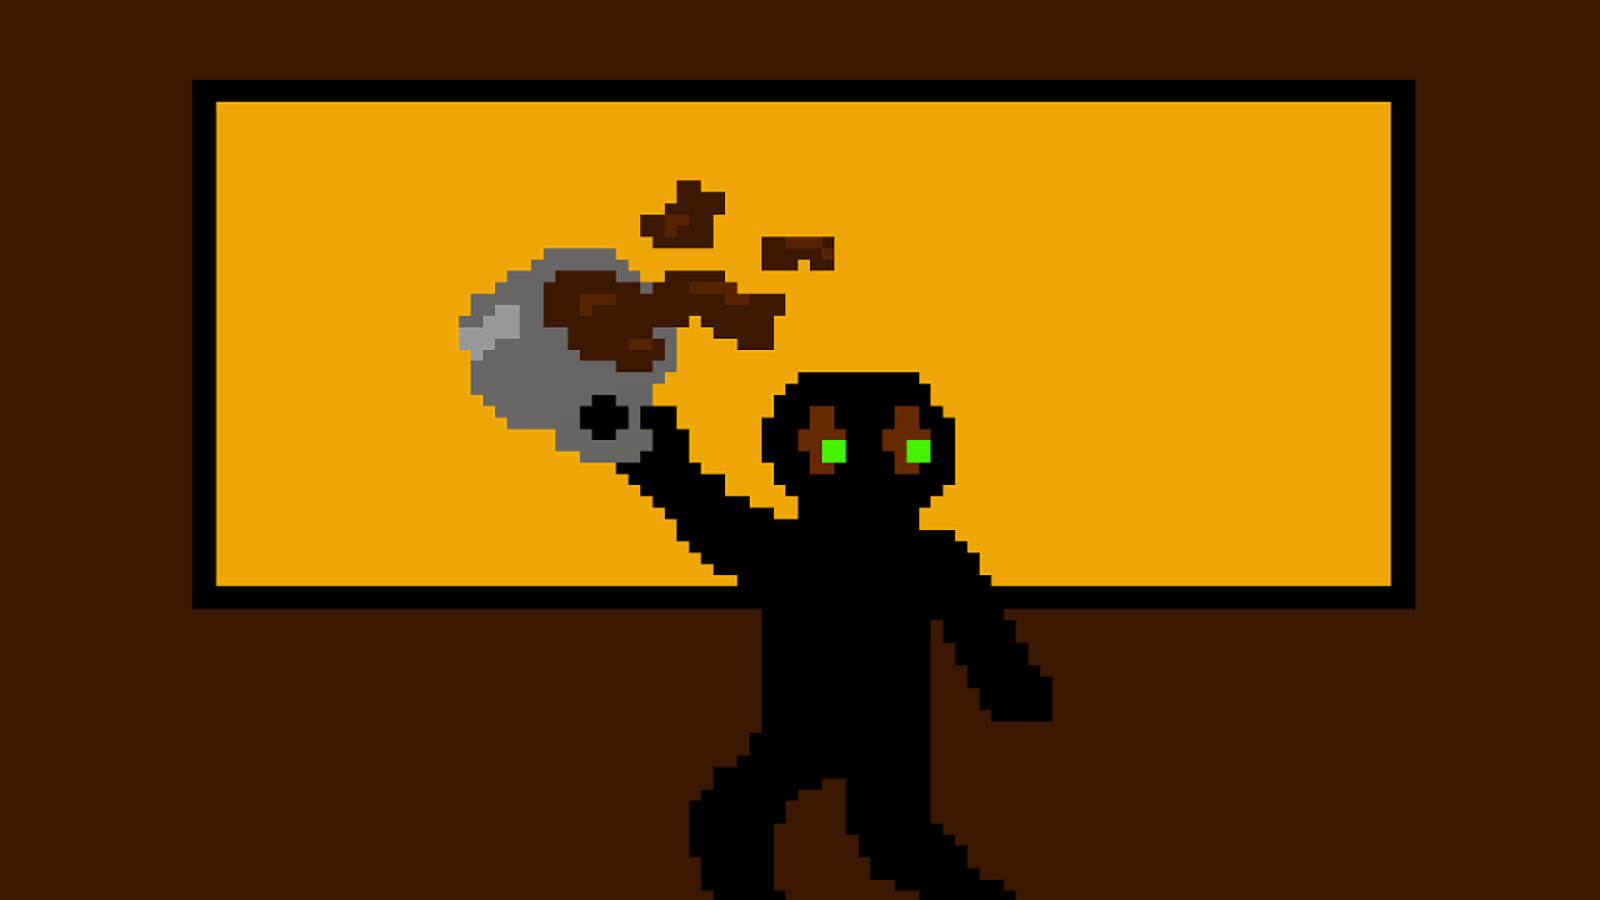
\includegraphics[width=15cm,height=15cm]{tdp005kravspe2c}
\subsection{Spelplan}
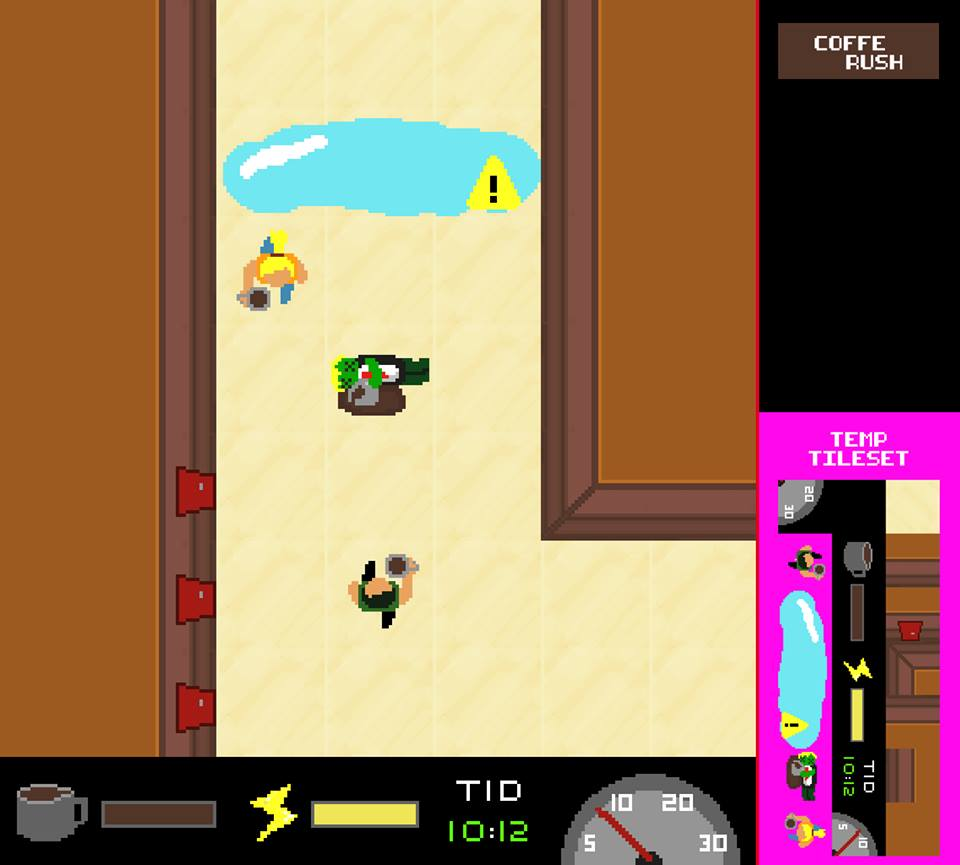
\includegraphics[width=15cm,height=15cm]{gamescreen2}

\section{Krav}
\subsection{Ska-krav}
1. Implementera ett sätt att skapa objekt enligt vår designspecifikation. \\
2. Skapa grunden för spelmotorn; dvs. skapa ett sätt att rita ut och uppdatera objekt.\\
3. Skapa en spelplan uppbyggd av enbart objekt (ingen tilemap, enbart x- och y-koordinater). \\
4. Implementera spelarkomponenten som håller reda på kaffe, uthållighet samt hjälpfunktioner för att modifiera dessa variablar.\\
5. Implementera styrkomponenten som tillåter spelaren att öka/sänka hastighet, hoppa samt gå mellan de olika spår med hjälp av de bestämda knapparna.\\
6. Implementera kollisionskomponenten som gör det möjligt för objekt kollidera med andra objekt som har denna komponent.\\
7. Implementera grunden för en hinderkomponent, som med hjälp av kollision komponenten kan få information om vilket objekt den kolliderar med.\\
8. Bygga upp hinderkomponenten för ett hala hinder; när spelaren kolliderar (och har för hög hastighet) ska spelaren trilla och förlora spelomgången.\\
9. Bygga upp hinderkomponenten för ett stilla stående hinder; när spelaren kolliderar ska spelaren tappa hastighet och en del av kaffet beroende på hastigheten.\\
10. Bygga upp hinderkomponenten för ett gående hinder; när spelaren kolliderar ska spelaren stanna upp i två sekunder.\\
11. Implementera basen för UI; dvs. ett sätt att rita ut UI komponenter på spelfönstret. \textbf{All UI har gjorts inne i GameScene. Inte som egna komponenter.}\\
12. Implementera kaffekomponent som tillåter objekt att hantera kaffe. (kommer användas i dagsläget enbart till spelaren)\\
18. Testa om hinderkomponenterna kan blandas med varandra för att skapa hindret `halt golv'. (stilla stående hinder + halt hinder)\\
%19. Testa om hinderkomponenterna kan blandas med varandra för att skapa hindret `gående student'. (gående hinder)\\
21. Slumpa fram olika hinder så att banan aldrig blir densamme som en annan spelomgång.\\
\subsection{Bör-krav}
13. Implementera uthållighetskomponent som tillåter objekt att bli tröttare och gå segare. (kommer användas i dagsläget enbart till spelaren)\\
14. Implementera UI komponent för kaffe; denna komponent ska rita upp en mätare på hur mycket kaffe finns kvar.\\
15. Implementera UI komponent för tid; denna komponent ska skriva ut passerad tid sedan start av spelomgången. (mm:ss)\\
16. Implementera UI komponent för hastighet; denna komponent ska rita upp en hastighetsmätare.\\

\subsection{Tilläggskrav}
22. Implementera ljudeffekter vid kaffespill.\\
23. Implementera ljudeffekter vid kollision med hinder.\\
24. Implementera bakgrundsmusik.\\
25. Implementera animerade sprites som används när spelaren går framåt.\\
26. Implementera animerade sprites som används när spelaren hoppar.\\
27. Implementera animerade sprites som används när spelaren trillar.\\
28. Implementera hindret `svart skärm' som används när spelaren kollar bort.\\



\section{Kravuppfyllelse}
\textit{Spelet ska simulera en värld som innehåller olika typer av objekt. Objekten ska ha olika beteenden och röra sig i världen och agera på olika sätt när de möter andra objekt.}
\begin{itemize}
    \item Punkter som uppfyller detta: 1,3, 4, 5, 6, 7, 8, 9, 10, 12, 13, 21.
\end{itemize} 
\textit{Det måste finnas minst tre olika typer av objekt och det ska finnas flera instanser av minst två av dessa. T.ex ett spelarobjekt och många instanser av två olika slags fiendeobjekt.}
\begin{itemize}
    \item Eftersom spelet kommer byggas upp på "component based design", så kommer det finnas otrolgit många kombinationer av objekt. Men vi kommer enbart använda dessa komponenter för att skapa tre hinder som kommer med i spelet från början. 
\end{itemize}
\textit{Ett beteende som måste finnas med är att figurerna ska röra sig över skärmen. Rörelsen kan följa ett mönster och/eller vara slumpmässig. Minst ett objekt, utöver spelaren ska ha någon typ av rörelse.}
\begin{itemize}
    \item Samma som ovan.
    \item Punkter som uppfyller detta specifikt: 5, 10.
\end{itemize}
\textit{En figur ska styras av spelaren, antingen med tangentbordet eller med musen. Du kan även göra ett spel där man spelar två stycken genom att dela på tangentbordet (varje spelare använder olika tangenter). Då styr man var sin figur.}
\begin{itemize}
    \item Punkter som uppfyller detta: 5.
\end{itemize}
\textit{Grafiken ska vara tvådimensionell.}
\begin{itemize}
    \item SFML används till detta.
\end{itemize}
\textit{Världen (spelplanen) kan antas vara lika stor som fönstret (du kan göra en större spelplan med scrollning, men det blir lite krångligare).}
\begin{itemize}
    \item Spelet kommer innehålla scrollning.
\end{itemize}
\textit{Det ska finnas kollisionshantering, det vill säga, det ska hända olika saker när objekten möter varandra, de ska påverka varandra på något sätt. T.ex kan ett av objekten tas bort, eller så kan objekten förvandlas på något sätt, eller så kan ett nytt objekt skapas. (Ett exempel på att skapa/ta bort objekt är när man i Space Invaders trycker på skjuta-knappen, t.ex en musknapp, då avfyras ett laserskott och skottet blir då en ny figur som skapas och placeras i världen, på en position vid laserkanonens mynning. Skottet rör sig framåt (uppåt) och om det träffar ett fiendeskepp tas både skottet och skeppet bort, om skottet kommer utanför spelplanen, dvs det missar, tas det endast bort.)}
\begin{itemize}
    \item Det finns genom att spelaren kan kollidera med de olika hinder och då händer en specifik grej till det hindret. T.ex. stöter spelaren på en liggande student och inte hoppar i tid, kommer kaffe spillas.
    \item Punkter som uppfyller detta: 6, 8, 9, 10.
\end{itemize}
\textit{Spelet måste upplevas som ett sammanhängande spel som går att spela!}
\begin{itemize}
    \item Är spelaren väldigt insatt på att få rekordet kommer denna att kunna spela hur länge som helst!
    \item Eftersom de olika hinder kommer vara slumpmässiga varje genomgång, kommer ingen spelsession vara samma som den förra!
\end{itemize}

\end{document}
